\documentclass[a4paper, 12pt]{extarticle}
\usepackage[dvipsnames]{xcolor}
\usepackage[top=70pt,bottom=70pt,left=48pt,right=46pt]{geometry}
\definecolor{header}{RGB}{252, 171, 16}
\definecolor{defenition}{RGB}{248, 51, 60}
\definecolor{main_title}{RGB}{43, 158, 179}
\definecolor{sub_header}{RGB}{68, 175, 105}
\usepackage[english, russian]{babel}
\usepackage[utf8]{inputenc}
\usepackage{amsmath}
\usepackage[most]{tcolorbox}
\usepackage{listings}
\usepackage{graphicx}
\usepackage{amsmath}
\usepackage{lettrine}
\title{\textcolor{main_title}{Инжекционные полупроводниковые лазеры}}
\author{Шмаков Владимир Евгеньевич - ФФКЭ гр. Б04-103}


\newtcolorbox{fequation}[1][]{ams equation*,size=small,#1}








\begin{document}
\maketitle



\section*{\textcolor{header}{Цель работы}}
\section*{\textcolor{header}{Теоретические сведения}}

\lettrine{\textcolor{defenition}{П}}{\textcolor{defenition}{олупроводниковые инжекционные лазеры}} 




\section*{\textcolor{header}{Методика}}

\subsection*{\textcolor{sub_header}{Оборудование}}


\subsection*{\textcolor{sub_header}{Экспериментальная установка}}

\section*{\textcolor{header}{Обработка экспериментальных данных}}
\subsection*{\textcolor{sub_header}{Выходные характеристики светодиода}}

\begin{figure}[htbp]
    \centering
    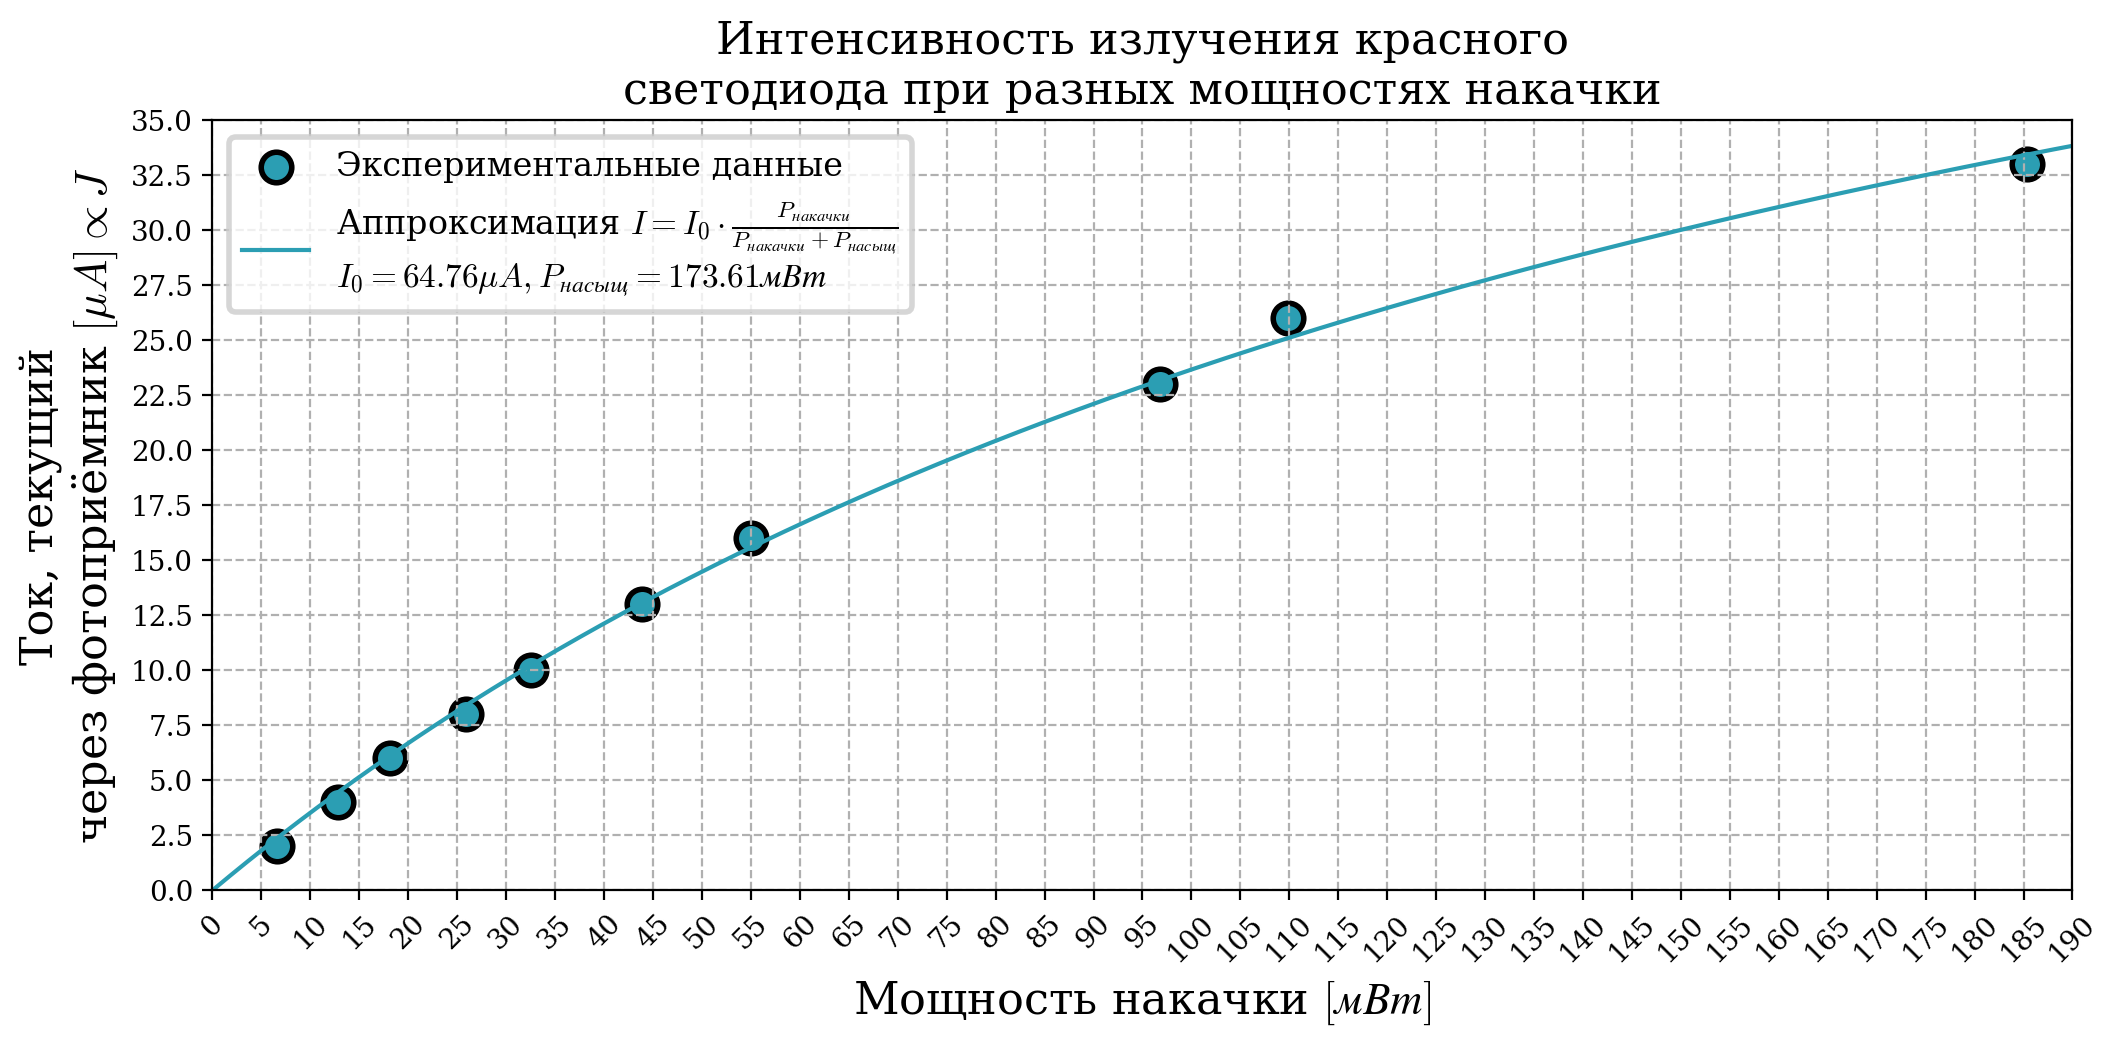
\includegraphics[width = 0.85\textwidth]{red_vc.png}
    \caption{Выходная характеристика красного светодиода}
    \label{fig:red_vc}
\end{figure}


\subsection*{\textcolor{sub_header}{Выходные характеристики полупроводникового лазера}}

\begin{figure}[htbp]
    \centering
    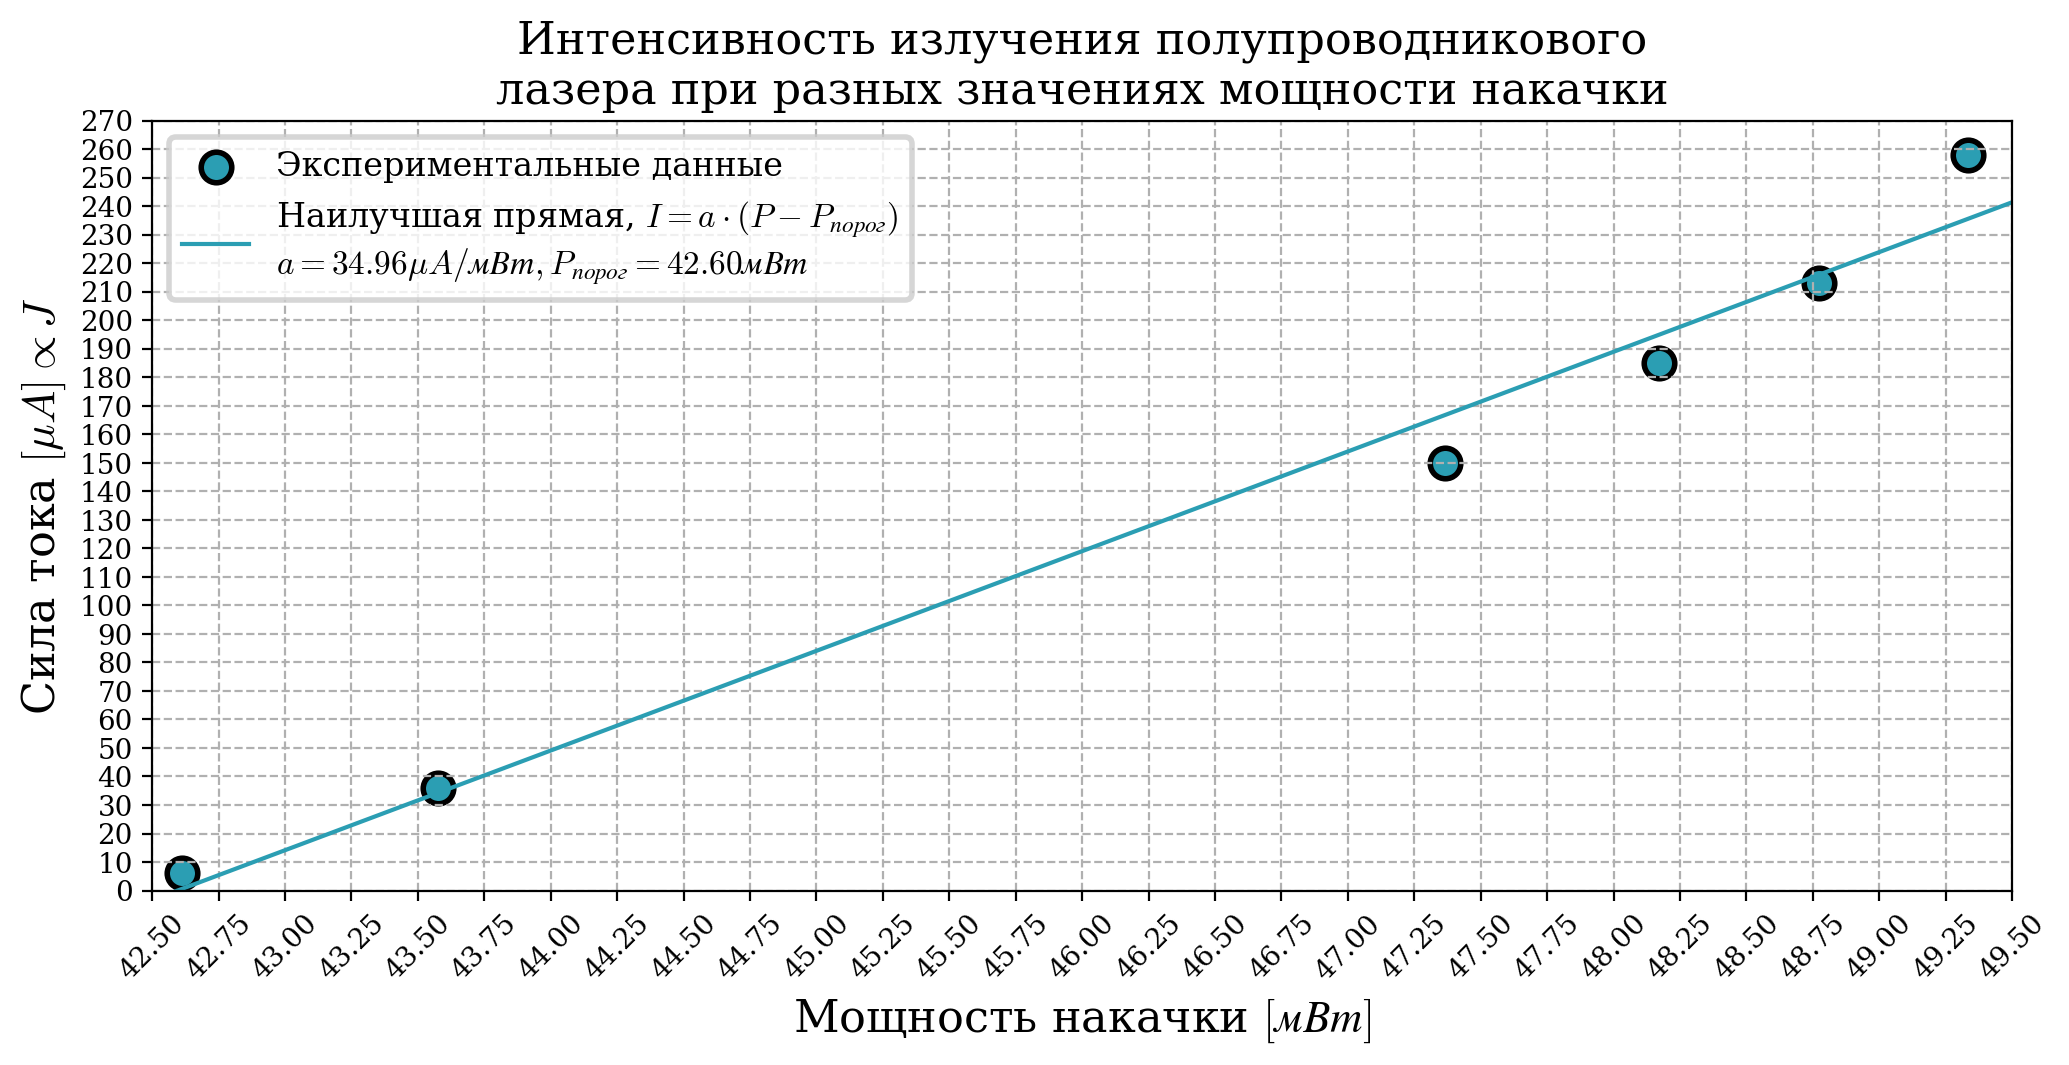
\includegraphics[width = 0.85\textwidth]{lazer.png}
    \caption{Выходная характеристика полупроводникового лазера}
    \label{fig:lazer}
\end{figure}

\subsection*{\textcolor{sub_header}{Спектры излучения светодиода}}


\begin{figure}[htbp]
    \centering
    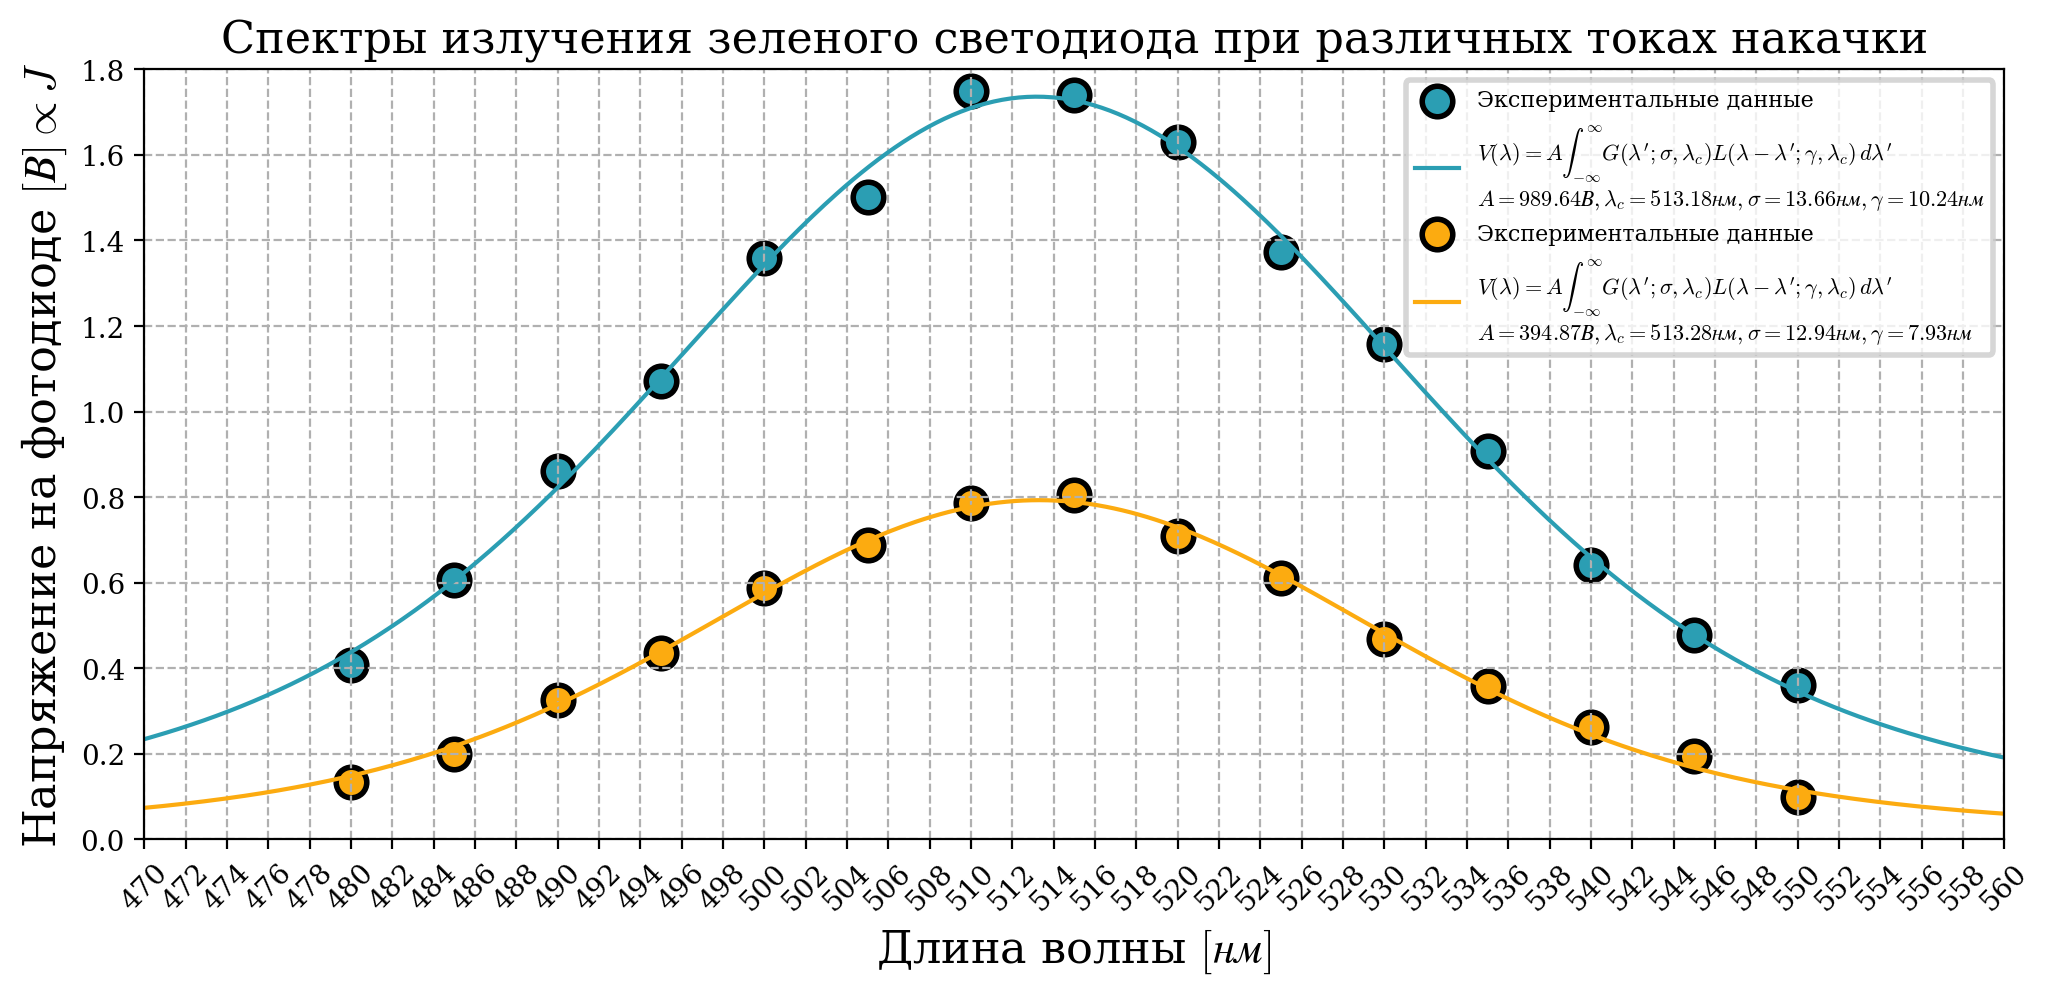
\includegraphics[width = 0.85\textwidth]{green.png}
    \caption{Выходная характеристика полупроводникового лазера}
    \label{fig:green}
\end{figure}


\begin{figure}[htbp]
    \centering
    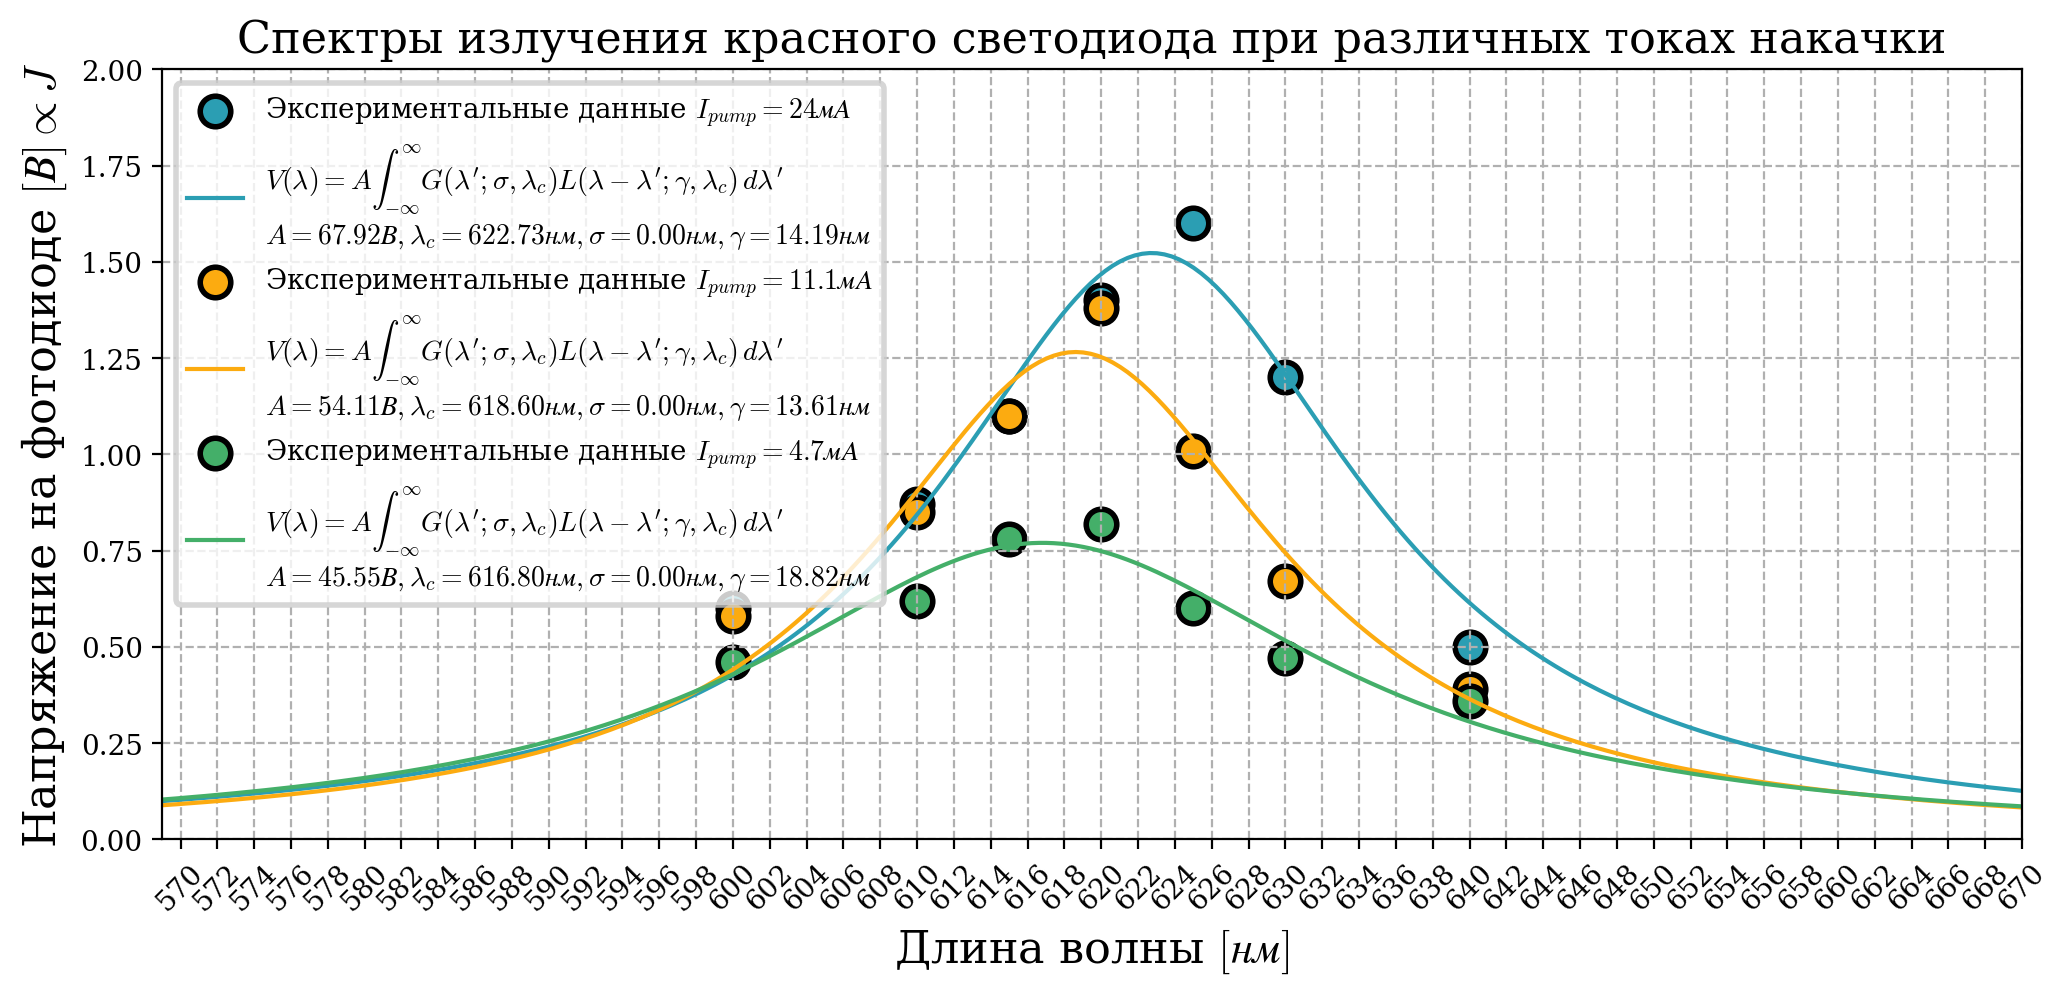
\includegraphics[width = 0.85\textwidth]{red.png}
    \caption{Выходная характеристика полупроводникового лазера}
    \label{fig:red}
\end{figure}


\begin{figure}[htbp]
    \centering
    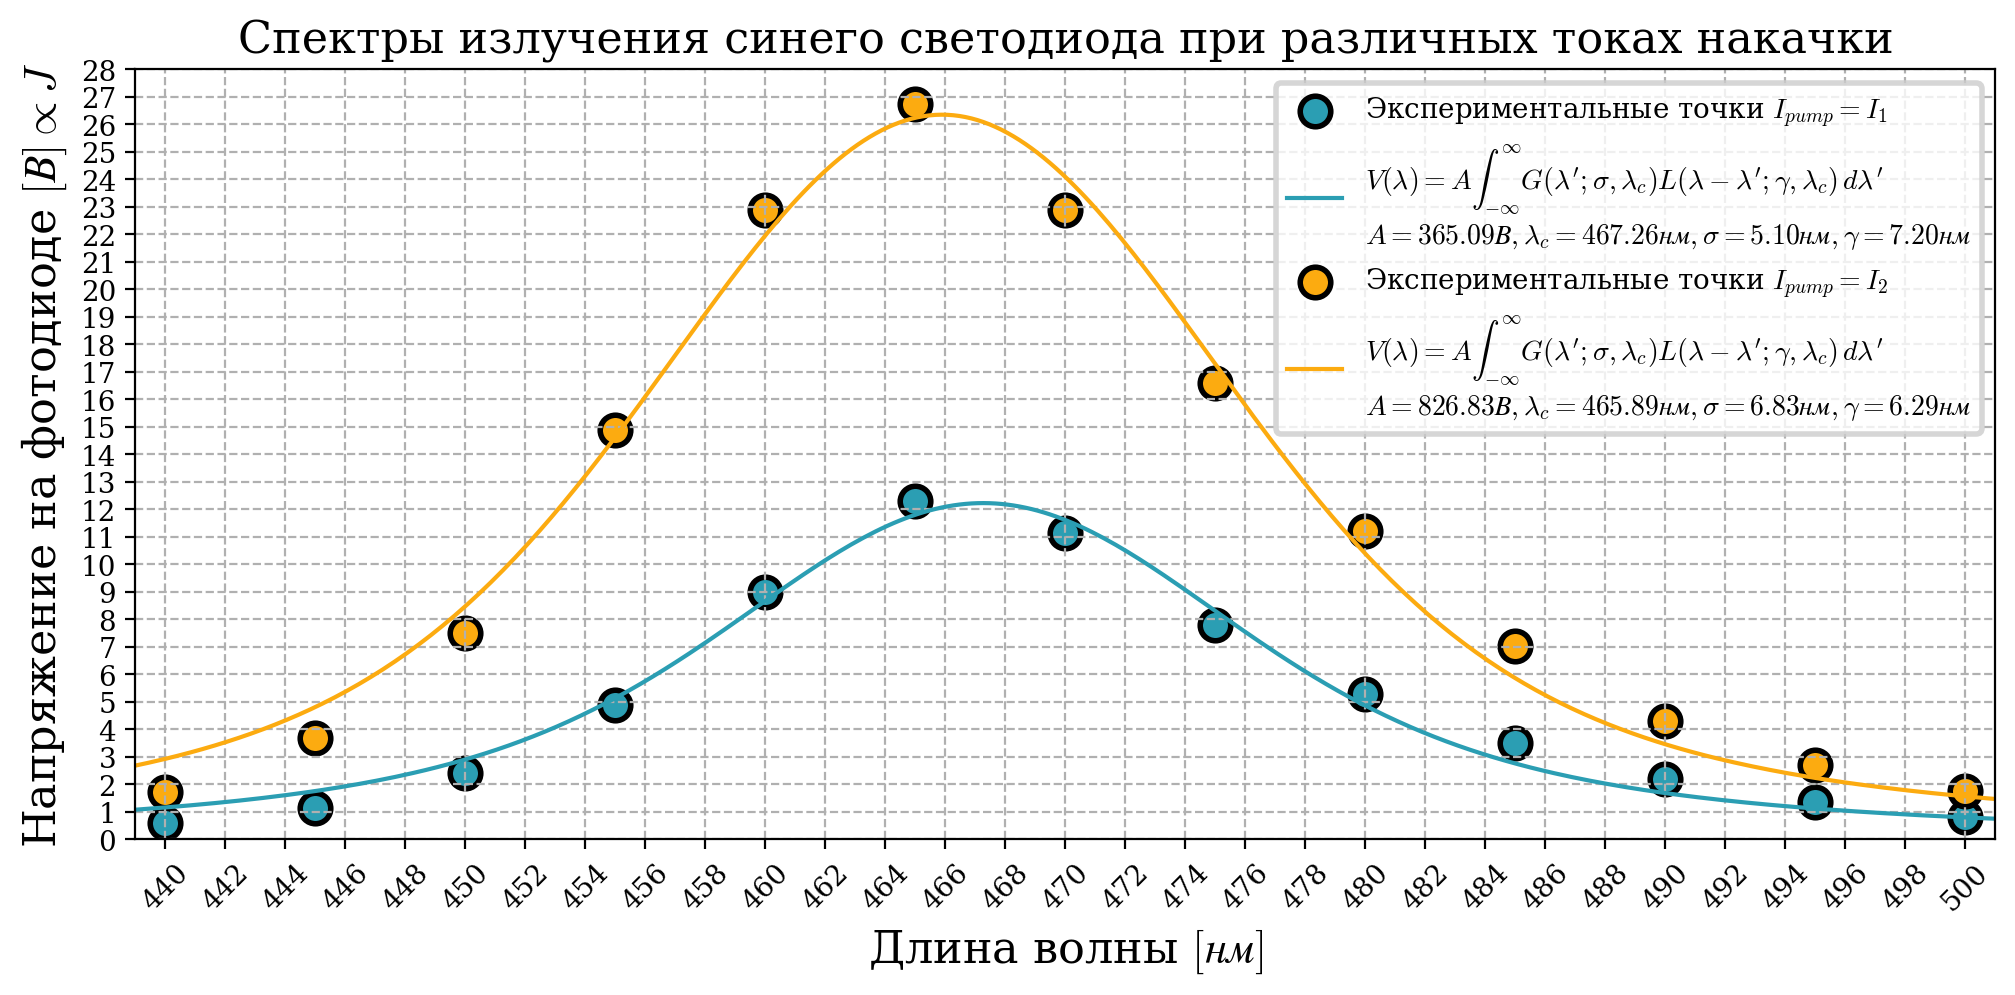
\includegraphics[width = 0.85\textwidth]{blue.png}
    \caption{Выходная характеристика полупроводникового лазера}
    \label{fig:blue}
\end{figure}






\section*{\textcolor{header}{Вывод}}






\end{document}
